\listfiles

% Formatierungsvorgaben der DHBW Mosbach:
% Weißes Paier, DIN A4 mit c.a. 70g/qm
% einseitig beschrieben
% je Zeile c.a. 70 Anschläge
% Zeilenabstand: 1,5 Zeilen
% Schriftgröße 12 Punkte bei Arial
% Randabstand: min. 25mm allseits
% Blocksatz
%
% Struktur:
% - Deckblatt
% - Sperrvermerk, wenn nötig
% - Erklärung über Selbstständige Arbeit
% - Zusammenfassung / Abstract
% - Inhaltsverzeichnis
% - Abkürzungsverzeichnis
% - Bildverzeichnis
% - Tabellenverzeichnis
% - Formelverzeichnis
% - Ausarbeitung Hauptteil
% - Literaturangaben
% - Anhang
%
% Bundesbank-Blau: 0x0062A1

\documentclass[ %
%draft,
12pt, 				% % % Schriftgröße 12 Punkte
a4paper,			% % % Papierformat DIN A4 210x297mm
oneside,			% % % Einseitiger Druck
openany, 			% % % Kann auf der linken oder rechten Seite beginnen (bei onside nicht notwendig)
titlepage,			% % % Der Titel kommt auf eine separate Seite
openbib,			% % % Verwendet openbib für die Literatur
listof=totoc,		% % % Zeigt Verzeichnisse Tabellenverzeichnis und Abbildungsverzeichnis im Inhalt an
bibliography=totoc,	% % % Zeigt das Literaturverzeichnis im Inhaltsverzeichnis an
numbers=noenddot,	% % % Lässt den abschließenden Punkt bei Abschnittsnummern weg
headsepline,		% % % Trennlinie zwischen Kopfzeile und Inhalt
headings=onelinechapter, % Kompakte Kapitelüberschriften
]{scrbook}			% % %  KOMA-Script für den Dokumententyp Buch


% % % Für eine saubere Encodierung und die deutsche Sprache
\usepackage[utf8]{inputenc}				% Lese UTF-8 Zeichen als Eingabe
\usepackage[T1]{fontenc}				% Schriftkodierung
\usepackage[ngerman]{babel}				% Deutsche Lokalisierung -> Standardbegriffe in Deutsch anstelle von Englisch
\usepackage{textcomp}					% Zusätzliche Symbole
%\usepackage[charter]{mathdesign}		% Mathefont

% root document
% !TeX root = ../Projektarbeit.tex

% Globale Variablen, insbesondere für die Titelseite
\def\title{Mars Science Laboratory Curiosity Rover}		% Titel der Arbeit
\def\titleFrontpage{Research Lab for Deep Learning \\ Mars Science Laboratory Curiosity Rover}
\def\doctype{Studienarbeit (T2\_000)}		% Art des Dokumentes, z.B. Studienarbeit, Bachelorarbeit, Bericht, ...
\def\studiengang{Angewandte Informatik}		% Studiengang
\def\author{Niklas Koopmann}				% Autor des Dokumentes
\def\matrikelNr{9742503}					% Autor des Dokumentes
\def\kursKurz{MOS-TINF17B}					% Autor des Dokumentes
\def\bearbeitungsZeit{24 Wochen}			% Bearbeitsungszeitraum
\def\ausbildungsfirma{Deutsche Bundesbank} 	% Ausbildungsfirma
\def\betreuerFirma{}						% Betreuer der Ausbildungsfirma
\def\betreuerDH{Prof. Dr. Carsten Müller}	% Betreuer der Dualen Hochschule
\def\abgabeDatum{\today}					% Abgabedatum der Arbeit

% % % Abstände bei Kapitelüberschriften ändern
\renewcommand*{\chapterheadstartvskip}{\vspace*{-5mm}}   % % % Freiraum vor der Überschrift
%\renewcommand*{\chapterheadendvskip}{\vspace{1cm}}      % % % Freiraum nach der Überschrift

% moved: Links im Dokument (to bottom)

\usepackage{scrhack}		 % % % Workaround für \float@addtolists Fehler

% % % Für das Literaturverzeichnis
\usepackage[
%style=authoryear-icomp,	 % % % Zitierstil - nur 1 verwenden!
style=numeric,				 % % % Zitierstil - nur 1 verwenden!
%style=authoryear,			 % % % Zitierstil - nur 1 verwenden!
isbn=true,                   % % % ISBN nicht anzeigen oder Verbergen, gleiches geht mit nahezu allen anderen Feldern
pagetracker=true,            % % % ebd. bei wiederholten Angaben (false=ausgeschaltet, page=Seite, spread=Doppelseite, true=automatisch)
maxbibnames=5,               % % % maximale Namen, die im Literaturverzeichnis angezeigt werden
maxcitenames=3,              % % % maximale Namen, die im Text angezeigt werden, ab 4 wird "u.a." nach den ersten Autor angezeigt
autocite=inline,             % % % regelt Aussehen für \autocite (inline=\parencite)
block=space,                 % % % kleiner horizontaler Platz zwischen den Feldern
backref=true,                % % % Seiten anzeigen, auf denen die Referenz vorkommt
backrefstyle=three+,         % % % fasst Seiten zusammen, z.B. S. 2f, 6ff, 7-10
date=short,                  % % % Datumsformat
backend=bibtex,	             % % % Beunutze das biber-Backend zur Erstellung an Stelle von bibtex
firstinits=true
]{biblatex}
\DefineBibliographyStrings{ngerman}{andothers={et\addabbrvspace al\adddot}}      % et al. statt u.a.
\setlength{\bibitemsep}{1em}	% % % Abstand zwischen den Literaturangaben
\setlength{\bibhang}{2em}		% % % Einzug nach jeweils erster Zeile
\addbibresource{literatur.bib}	% % % Literaturdatenbank einlesen
\bibliography{literatur}        % % % Literaturdatenbank einlesen

\usepackage{xcolor}
\definecolor{monospacebackgroundcolor}{RGB}{230,230,240}
\definecolor{monospacecolor}{RGB}{50,0,0}
\definecolor{bbkblau}{RGB}{0,98,161}
\definecolor{bbkgrau}{RGB}{219,219,219}
\definecolor{bbkhellgruen}{RGB}{192,217,110}
\definecolor{bbkdunkelgruen}{RGB}{134,195,135}
	
% % % Für das Abkürzungsverzeichnis:
\usepackage[printonlyused]{acronym}



% % % Schriften und Layout
\usepackage{lmodern}		% Standardschriftart von Latex
\usepackage[expansion=true, protrusion=true]{microtype}	% Abstände verbessern
\usepackage[babel,german=quotes]{csquotes}



% % % Für die Einbindung von Grafiken
\usepackage{graphicx}	% Für Grafiken allgemein
\usepackage{epstopdf}	% Für *.eps-Grafiken mit pdfLaTeX
%\usepackage{svg}		% Für *.svg-Grafiken
\usepackage{caption}	% Verbesserungen bei der Beschriftung von Bildern und Tabellen
%\usepackage{float}		% Verbesserung für fließende Objekte
%\usepackage[extendedchars, encoding, multidot, space, filenameencoding=utf8]{grffile}
\usepackage{wrapfig}
\usepackage{pdfpages}



% % % Für Tabellen
\usepackage{typearea}	
\usepackage{array}		% Basispaket für Tabellen
\usepackage{ltxtable}	% Erweiterung für Tabellen
\usepackage{booktabs}	% Verbesserung für die Darstellung von Tabellen
\usepackage{enumitem}
\usepackage{makecell}	% \thead-Befehl in Tabellen
\usepackage{multirow}
\usepackage{hhline}


% % % URLs ordentlich darstellen
\usepackage{url}

% % % Blindtextgenerator, wird in Dokumenten normalerweise nich benötigt
\usepackage{blindtext}

% % % Seitenabmessungen und Randabstand
\usepackage[ %
%width=210.00mm, height=297.00mm, %
left=2.80cm, right=2.60cm, top=2.60cm, bottom=2.60cm]{geometry}



% % % Für Mathe:
\usepackage{amsmath}	% Mathematische Konstrukte
\usepackage{amsfonts}	% Mathematische Schriftarten
\usepackage{amssymb}	% Mathematische Symbole
\usepackage{gensymb}	% noch mehr Symbole


% % % Für Quelltexte
\usepackage{listings}
\usepackage{color}

% % % Bäume
\usepackage{tikz}
\usetikzlibrary{positioning}
\usetikzlibrary{trees}
\usetikzlibrary{matrix}


\definecolor{colordcodebackground}{rgb}{0.9,0.9,0.9}
\definecolor{colorcodegreen}{rgb}{0,0.4,0}
\definecolor{colorcodegrey}{rgb}{0.4,0.4,0.4}
\definecolor{colorcodestring}{rgb}{0.58,0.0,0.82}
\definecolor{colorcodekeys}{rgb}{0.0,0.0,0.8}
\definecolor{colorcoderule}{rgb}{0.65,0.65,0.65}

\lstset{ %
	backgroundcolor=\color{colordcodebackground},   % choose the background color; you must add \usepackage{color} or \usepackage{xcolor}
	basicstyle=\ttfamily\footnotesize,  % the size of the fonts that are used for the code
	breakatwhitespace=false,         % sets if automatic breaks should only happen at whitespace
	breaklines=true,                 % sets automatic line breaking
	captionpos=b,                    % sets the caption-position to bottom
	commentstyle=\color{colorcodegreen},    % comment style
	deletekeywords={...},            % if you want to delete keywords from the given language
	escapeinside={\%*}{*)},          % if you want to add LaTeX within your code
	extendedchars=true,              % lets you use non-ASCII characters; for 8-bits encodings only, does not work with UTF-8
	frame=single,	                 % adds a frame around the code
	keepspaces=true,                 % keeps spaces in text, useful for keeping indentation of code (possibly needs columns=flexible)
	keywordstyle=\color{colorcodekeys},       % keyword style
	%language=Java,                	 % the language of the code
	otherkeywords={},           % if you want to add more keywords to the set
	numbers=left,                    % where to put the line-numbers; possible values are (none, left, right)
	numbersep=5pt,                   % how far the line-numbers are from the code
	numberstyle=\color{colorcodegrey}, 	 % the style that is used for the line-numbers
	rulecolor=\color{colorcoderule},         % if not set, the frame-color may be changed on line-breaks within not-black text (e.g. comments (green here))
	showspaces=false,                % show spaces everywhere adding particular underscores; it overrides 'showstringspaces'
	showstringspaces=false,          % underline spaces within strings only
	showtabs=false,                  % show tabs within strings adding particular underscores
	stepnumber=1,                    % the step between two line-numbers. If it's 1, each line will be numbered
	stringstyle=\color{colorcodestring},     % string literal style
	tabsize=4,	                   	 % sets default tabsize to 2 spaces
	title=\lstname,                   % show the filename of files included with \lstinputlisting; also try caption instead of title
	float
} % max 73 Zeichen je Zeile
\renewcommand{\lstlistlistingname}{Quelltextverzeichnis}
\renewcommand{\lstlistingname}{Quelltext}
% http://tex.stackexchange.com/questions/89574/language-option-supported-in-listings
\lstdefinelanguage{js}{
	keywords={break, case, catch, continue, debugger, default, delete, do, else, false, finally, for, function, if, in, instanceof, new, null, return, switch, this, throw, true, try, typeof, var, void, while, with},
	morecomment=[l]{//},
	morecomment=[s]{/*}{*/},
	morestring=[b]',
	morestring=[b]",
	ndkeywords={class, export, boolean, throw, implements, import, this},
	keywordstyle=\color{blue}\bfseries,
	ndkeywordstyle=\color{darkgray}\bfseries,
	identifierstyle=\color{black},
	commentstyle=\color[rgb]{0,0.4,0}\ttfamily,
	stringstyle=\color[rgb]{0.7,0.0,0.8}\ttfamily,
	sensitive=true
}


% % % Kopf- und Fußzeile
\usepackage{scrpage2}
\pagestyle{scrheadings}
\clearscrheadings
%\ifoot{\leftmark}{\leftmark}
\ifoot{}{}
%\ihead{\rightmark}{\rightmark} % % % Rightmark oben links
\ohead{\rightmark}{\rightmark} % % % Rightmark oben links
%\ohead[\pagemark]{\pagemark}  % % % Seitenzahl oben rechts
\ofoot[\pagemark]{\pagemark}   % % % Seitenzahl unten rechts
\cfoot[]{}					   % % % Leere Mitte unten
\automark[section]{chapter}	   % % % [Leftmark] und {Rightmark} setzen







% % % Layout-Optionen:
\renewcommand*{\headfont}{\normalfont}
%\renewcommand*{\multicitedelim}{\addsemicolon\space}
%\renewcommand*{\headrulewidth}{0pt}
\renewcommand*{\arraystretch}{1.5}



% % % Globaler Zeilenabstand: 1,5-zeilig
\usepackage[onehalfspacing]{setspace}
%\setlength{\parskip}{1.5em}
\recalctypearea



% % % Makrobefehle

% Verweis 
% Befehl \see{label}
% #1 : reflabel
\def\see#1{ %
	\text{($\rightarrow$}\space\nameref{#1}\space\text{auf S.}\space\pageref{#1}\text{)}
}

% Bild
% Befehl \bild{Bilddatei}{Beschriftung}{label}
% #1 : Bilddatei
% #2 : Beschriftung / Bildunterschrift
% #3 : Label
\def\bild#1#2#3{ %
	\begin{figure}[h]
		\centering
		\includegraphics[width=0.9\textwidth]{#1}
%		\vspace{5mm}
		\caption{#2}
		\label{#3}
	\end{figure}
}

% Code
% Befehl \code{Quelldatei}{Beschriftung}{label}{Sprache}
\def\code#1#2#3#4{ %
	\begin{center}
	\centering
	\lstset{language=#4,caption={#2},label=#3}
	\singlespacing
	\lstinputlisting[language=#4]{#1}
	\end{center}
}

% Monospace
% Befehl \mono{Text}
\newcommand{\mono}[1]{
	\texttt{\colorbox{monospacebackgroundcolor}{\textcolor{monospacecolor}{#1}}}
	%\texttt{\textcolor{monospacecolor}{#1}}
	%\texttt{#1}
}

\newcommand{\signature}[1]{%
	\parbox{\textwidth}{
		%\centering #3 \today\\
		%\vspace{2cm}
		
		\parbox{7cm}{
			\centering
			\rule{6cm}{1pt}\\
			Ort, Datum 
		}
		\hfill
		\parbox{7cm}{
			\centering
			\rule{6cm}{1pt}\\
			#1
		}
	}
} 

% wechselnde Footnotes (Anmerkungen als Buchstaben)
% usage \ftnote{Basistext}{Fußnotentext}{Index der Fußnote}
\newcommand{\ftnote}[3]{
	\renewcommand{\thefootnote}{\alph{footnote}}
	#1\footnote[#3]{#2}
	\renewcommand{\thefootnote}{\arabic{footnote}}
}

%% better: (general command to vertically center horizontal material)
\newcommand*{\vcenteredhbox}[1]{\begingroup
	\setbox0=\hbox{#1}\parbox{\wd0}{\box0}\endgroup}


% % % Links im Dokument erzeugen
%\usepackage[colorlinks, allcolors=blue, breaklinks]{hyperref}
\usepackage[colorlinks, allcolors=black, breaklinks]{hyperref}
%\usepackage[colorlinks, linkcolor = black, citecolor = black, filecolor = black, urlcolor = blue]{hyperref} 

\begin{document}
	
% % % Alle Quellen aus literatur.bib ins Literaturverzeichnis schreiben% \nocite{*} % % % Auskommentieren, sodass nur verwendete Quellen gelistet werden

\frontmatter
\pagenumbering{Roman}
\begin{titlepage}

\begin{center}
	\setlength{\voffset}{-15mm}
	
\includegraphics[height=20mm]{general/bundesbank-logo.pdf}
	\hspace{60mm}
	
\includegraphics[height=20mm]{general/logo-dhbw-mos.jpg}

	\vspace{50pt}
	
	\LARGE \titleFrontpage
	\vspace{20pt}
	
%	\vspace{20pt}
	\Large \doctype \\[1.5mm]
	\small für die Prüfung zum \\
	\large Bachelor of Science
	
	\vspace{15pt}
	
	\normalsize des Studiengangs \studiengang \space an der \\
	\normalsize Dualen Hochschule Baden-Württemberg Mosbach
	
	\vspace{20pt}
	
	\small von \\
	\large \author
\end{center}

\vspace{25pt}

\begin{table}[ht]
	\centering
	\begin{tabular}{ll}
	\small Abgabedatum							& \abgabeDatum			 \\
	\small Bearbeitungszeitraum					& \bearbeitungsZeit		 \\
	\small Matrikelnummer, Kurs					& \matrikelNr, \kursKurz \\
	\small Ausbildungsunternehmen				& \ausbildungsfirma		 \\
	\small Gutachter der Dualen Hochschule		& \betreuerDH			 \\
	\end{tabular}
\end{table}

\end{titlepage}
%\chapter*{Sperrvermerk}
%Die vorliegende Arbeit beinhaltet interne vertrauliche Informationen der Deutschen Bundesbank. Sie ist nur für die Beteiligten am Begutachtungs- und Evaluationsprozess bestimmt.

%Die Weitergabe des Inhalts der Arbeit im Gesamten oder in Teilen sowie das Anfertigen von Kopien oder Abschriften - auch in digitaler Form - sind grundsätzlich untersagt. Ausnahmen bedürfen der schriftlichen Genehmigung der Deutschen Bundesbank
%Dieser Sperrvermerk gilt zum Datum.

Die vorliegende \doctype \ \enquote{\title} enthält vertrauliche Daten der Deutschen Bundesbank. 
Die Arbeit darf nur den Gutachtern sowie befugten Mitgliedern des Prüfungsausschusses zugänglich gemacht werden. 

\noindent
Eine Veröffentlichung und Vervielfältigung der Arbeit ist -- auch in Auszügen -- nicht gestattet.
Eine Einsichtnahme der Arbeit durch Unbefugte bedarf einer ausdrücklichen Genehmigung der Deutschen Bundesbank.

\noindent
Dieser Sperrvermerk gilt unbegrenzt.

\vspace{3cm}
Ort, Datum 
\hspace{5cm}
Unterschrift


\chapter*{Ehrenwörtliche Erklärung}
%Gemäß §5 (3) der "`Studien- und Prüfungsordnung der DHBW Technik"' vom 22. September 2011 erkläre ich:\\[1em]
%Ich habe die Vorliegende Arbeit selbstständig verfasst und keine anderen als die angegebenen Quellen und Hilfsmittel verwendet
\fbox{\parbox{\textwidth}{
		%\center{Erklärung}
		\vspace{15pt}
		\begin{addmargin}{15pt}
		Erklärung
		\vspace{15pt}
		
		Ich versichere hiermit, dass ich meine Bachelorarbeit (bzw. Studien- und Projektarbeit) mit dem Thema \enquote{\title} selbstständig verfasst und keine anderen als die angegebenen Quellen und Hilfsmittel benutzt habe.
		
		\noindent
		Ich versichere zudem, dass die eingereichte elektronische Fassung mit der gedruckten Fassung
		übereinstimmt. *
		
		\vspace{15pt}
		\noindent
		\footnotesize * falls beide Fassungen gefordert sind
		\end{addmargin}
		
		\normalsize
		\vspace{3cm}
		\signature{Niklas Koopmann}
	}
}

\vspace{1cm}

\begin{center}
	\parbox{0.8\textwidth}{
		\begin{description}
			\item[Hinweis:] Aus Gründen der besseren Lesbarkeit wird in dieser Arbeit auf die gleichzeitige Verwendung männlicher und weiblicher Sprachform verzichtet (\textit{generisches Maskulinum}). Sämtliche Personenbezeichnungen gelten gleichwohl für beiderlei Geschlecht.
		\end{description}
	}
\end{center}
\chapter{Abstract}
\label{sec:abstractenglish}

% TEXT

\vspace{1cm}

\begingroup
\renewcommand{\pagebreak}{}
\renewcommand{\clearpage}{}
\chapter*{Zusammenfassung}
\label{sec:abstract}

% TEXT

\endgroup
\tableofcontents
% Usage:
% \ac{KDE}		Gibt bei der ersten Verwendung 
%		die Langform mit der Abkürzung in Klammern aus, 
%		ab dann stets die Kurzform.
% \acs{KDE}		Gibt die Abkürzung aus
% \acf{KDE}		Gibt die Langform und die Kurzform aus
% \acl{KDE}		Gibt die Langform ohne Kurzform aus
% \acp{JDK}		Wie oben, allerdings im Plural
% \acsp{JDK}	Wie oben, allerdings im Plural
% \acfp{JDK}	Wie oben, allerdings im Plural
% \aclp{JDK}	Wie oben, allerdings im Plural
% \acrodefplural{VM}[VMs]{Virtuelle Maschinen}

\chapter{Abkürzungsverzeichnis}
\begin{acronym}[WHATWG ]
\setlength{\itemsep}{-\parsep}
\acro{ad}[AD]{Active Directory}
\acro{adfs}[AD FS]{Active Directory Federation Services}
\acro{alsa}[ALSA]{Advanced Linux Sound Architecture}
\acro{api}[API]{Application Programming Interface}
\acro{aws}[AWS]{Amazon Web Services}
\acro{bafin}[BaFin]{Bundesanstalt für Finanzdienstleistungsaufsicht}
\acro{bdsg}[BDSG]{Bundesdatenschutzgesetz}
\acro{bmf}[BMF]{Bundesministerium der Finanzen}
\acro{bsi}[BSI]{Bundesamt für Sicherheit in der Informationstechnik}
\acro{ci}[CI]{Continuous Integration}
\acro{cifs}[CIFS]{Common Internet File System}
\acro{cli}[CLI]{Command Line Interface}
\acro{dhbw}[DHBW]{Duale Hochschule Baden-Württemberg}
\acro{dmz}[DMZ]{Demilitarisierte Zone}
\acro{dn}[DN]{Distinguished Name}
\acro{dns}[DNS]{Domain Name System}
\acro{dps}[DPS]{Directory and Password Synchronization}
\acro{dsgvo}[DSGVO]{Datenschutz-Grundverordnung}
\acro{ee}[EE]{Execution Environment}
\acro{ese}[ESE]{Extensible Storage Engine}
\acro{eszb}[ESZB]{Europäisches System der Zentralbanken}
\acro{ezb}[EZB]{Europäische Zentralbank}
\acro{fqdn}[FQDN]{Fully Qualified Domain Name}
\acro{gpio}[GPIO]{General Purpose Input/Output}
\acro{hat}[HAT]{Hardware Attached on Top}
\acro{hdmi}[HDMI]{High Definition Multimedia Interface}
\acro{hsv}[HSV]{Hue, Saturation, Value}
\acro{http}[HTTP]{Hypertext Transfer Protocol}
\acro{iaas}[IaaS]{Infrastructure as a Service}
\acro{ide}[IDE]{Integrated Development Environment}
\acro{iso}[ISO]{International Organization for Standardization}
\acro{lan}[LAN]{Local Area Network}
\acro{ldap}[LDAP]{Lightweight Directory Access Protocol}
\acro{mfa}[MFA]{Multi-Factor Authentication}
\acro{nasa}[NASA]{National Aeronautics and Space Administration}
\acro{nist}[NIST]{National Institute of Standards and Technology}
\acro{nzb}[NZB]{Nationale Zentralbank}
\acroplural{nzb}[NZBn]{Nationale Zentralbanken}
\acro{paas}[PaaS]{Platform as a Service}
\acro{phs}[PHS]{Password Hash Synchronization}
\acro{pin}[PIN]{Personal Identification Number}
\acro{pta}[PTA]{Pass-Through Authentication}
\acro{rest}[REST]{Representational State Transfer}
\acro{rfc}[RFC]{Request for Comments}
\acro{rgb}[RGB]{Rot, Grün, Blau}
\acro{saas}[SaaS]{Software as a Service}
\acro{sla}[SLA]{Service Level Agreement}
\acroplural{sla}[SLAs]{Service Level Agreements}
\acro{ssis}[SSIS]{SQL Server Integration Services}
\acro{sso}[SSO]{Single Sign-On}
\acro{url}[URL]{Uniform Resource Locator}
\acro{vba}[VBA]{Visual Basic for Applications}
\acro{vc}[VC]{Virtual Client}
\acroplural{vc}[VCs]{Virtual Clients}
\acro{vpn}[VPN]{Virtual Private Network}
\acro{wins}[WINS]{Windows Internet Name Service}
\acro{xml}[XML]{eXtensible Markup Language}
\end{acronym}
\listoffigures
%\listoftables
%\chapter{Formelverzeichnis}
\begin{singlespace}
\begin{description}
\item[$\mathbb{N}$] Menge der natürlichen Zahlen
\end{description}
\end{singlespace}
\lstlistoflistings


\mainmatter
\pagenumbering{arabic}

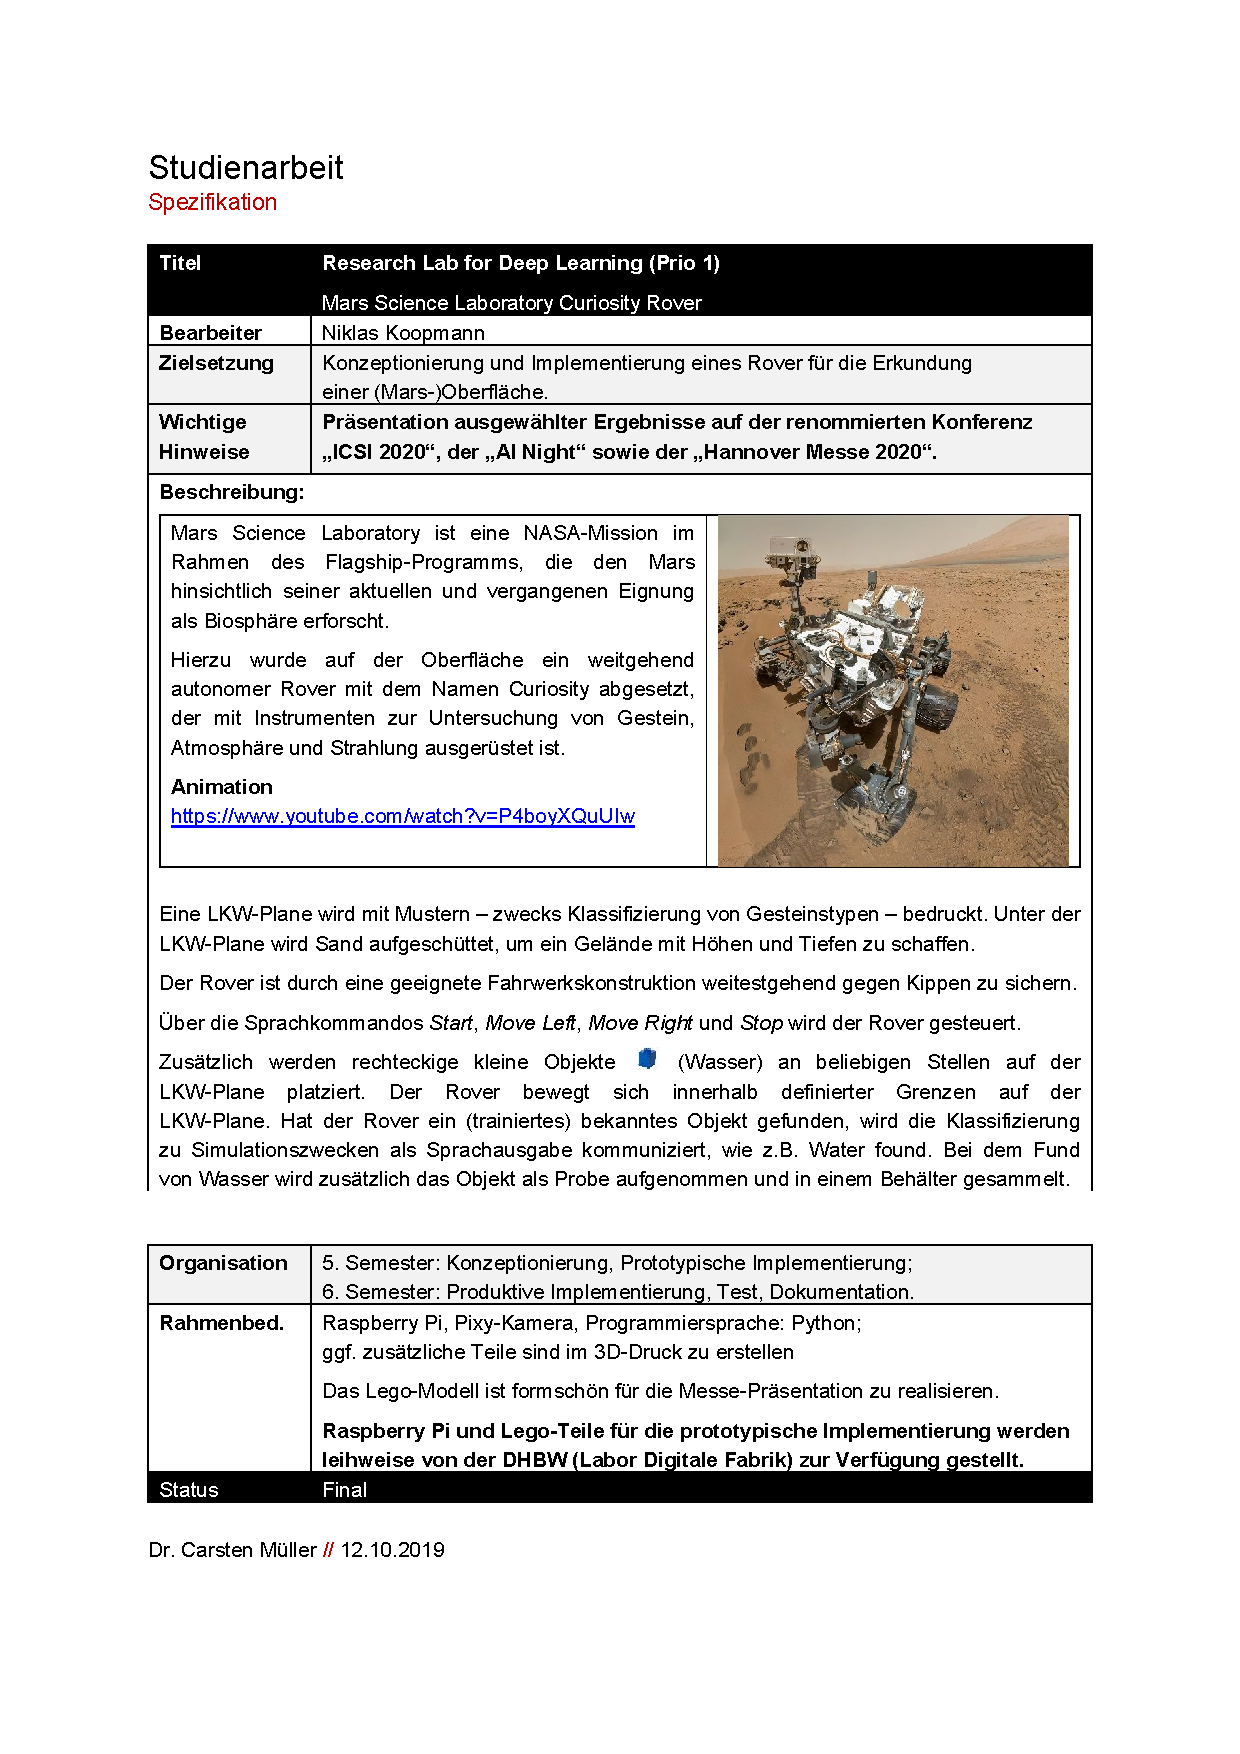
\includepdf[scale=0.8, pages=1, offset=0 -1cm, pagecommand={\chapter{Spezifikation} \label{chp:spezifikation}}]{content/spec.pdf}
\includepdf[scale=0.8, pages=2-, offset=0 -1cm, pagecommand={}]{content/spec.pdf}

\section{Motivation}
\label{sec:motivation}

Am 6. August 2012 landete der Rover \textit{Curiosity} als Teil der Mission \textit{Mars Science Laboratory} der US-amerikanischen Raumfahrtbehörde \acf{nasa} im Gale-Krater auf dem Mars \cite{vasavada2014}.
Seither hat er rund $21{,}93$ Kilometer zurückgelegt (Stand: Sol 2695) \cite{nasa2020} und die Landschaft entlang der Fahrtstrecke auf vielfältige Weise im Hinblick auf ihre frühere und aktuelle Eignung als Lebensraum für Organismen untersucht.
Ein wichtiger Aspekt für den Nachweis der Existenz von Lebewesen ist das Vorhandensein flüssigen Wassers \cite{nasa2013}, dessen Rückstände der Rover mithilfe eines aktiven Neutronenspektrometers in Mineralien nachzuweisen versucht. \cite{vasavada2014}

Um weite Strecken im schroffen, unebenen Gelände der Marsoberfläche zurücklegen zu können, ist \textit{Curiosity} mit einem komplexen, sechsrädrigen Antriebs- und Federungssystem ausgestattet.
Das Fahrwerk ist nach dem Rocker-Bogie-System der \acs{nasa} aufgebaut, um Hindernisse bis zu einer Höhe des Raddurchmessers von $0{,}5\ m$ überwinden zu können \cite{arvidson2013}.
Eine solche Aufhängung ermöglicht dem Rover eine hohe Geländegängigkeit ohne den Einsatz von Achsen und erlaubt der Verbindung der hinteren Räder beider Seiten eine freie Drehung um den Verbindungspunkt zur Hauptstrebe, an der auch das jeweilige Vorderrad montiert ist \cite{bickler1998}. 

% TODO Weitere Ausführungen

Dieses Projekt (Mars Science Laboratory Curiosity Rover) wird im Rahmen des Research Lab for Deep Learning der Dualen Hochschule Baden-Württemberg (\acsu{dhbw}) zeitgleich mit der Erforschung schwarmbasierter Logistikabläufe durchgeführt.
Langfristig soll das Ergebnis unter anderem zum Zwecke einer schwarmbasierten Erkundung marsähnlicher Landschaften weiterentwickelt werden können.

\section{Aufgabenstellung}
\label{sec:aufgabe}

Ziel dieser Arbeit ist die \glqq Konzeptionierung und Implementierung eines Rover für die Erkundung einer (Mars-)Oberfläche\grqq\ \cite{mueller2019}.
Die Suche nach Wasser wird dabei ebenfalls abgebildet und soll mithilfe der visuellen Erkennung blauer LEGO-Steine simuliert werden.
Zusätzlich ist das Antriebskonzept des \textit{Curiosity}-Rovers originalgetreu nachzubilden: Es sollen sechs angetriebene Räder installiert sein, von denen vier gelenkt werden.
Eine grundlegende mechanische Federung soll die Geländetauglichkeit steigern.

In einzelnen Punkten ist nachträglich einvernehmlich von der Spezifikation abgewichen worden:
Der Rover muss keine Wasserobjekte aufsammeln können.
Wenn ein Wasserobjekt erkannt wird, soll dies lediglich über die Sprachausgabe verkündet werden.
Der Fokus der Entwicklung ist von der Geländetauglichkeit hin zur Stabilität und Formschönheit gerückt worden.
Das klassische Rocker-Bogie-Fahrwerk wird im Sinne der Originaltreue in leicht abgewandelter Form verbaut (siehe dazu Abschnitt \ref{sec:seitenansicht}).

% TODO REMOVE LITERATURE TESTS
Literatur-Test:
\cite{yamanoor2017}
\cite{horan2013}
\cite{molloy2016}
\cite{donat2018}
\cite{halfacree2019}
\cite{mcmanus2017}
\cite{cox2014}
\chapter{Systeme, Infrastruktur und Services}
\label{chp:grundlagen}




\chapter{Fazit}
\label{chp:fazit}

Im Rahmen dieser Studienarbeit ist ein weitgehend funktionsfähiges und nutzbares Mars-Rover-Modell nach dem realen Vorbild, dem Curiosity-Rover der \acs{nasa}, in Form einer Machbarkeitsstudie (Proof of Concept) von Grund auf entwickelt worden.
Das Ergebnis entspricht gänzlich den in Kapitel \ref{chp:spezifikation} definierten und im Verlauf der Entwicklung angepassten Anforderungen.
Besonderes Augenmerk wurde bereits bei der Konzeption des Rovers auf die originalgetreue und formschöne Abbildung wichtiger Komponenten wie dem Rocker-Bogie-Fahrwerk mit sechsrädrigem Antriebssystem und der Kamerapositionierung im Kopf gelegt.
Zudem sind charakteristische Strukturelemente von Curiosity, zum Beispiel der stets leicht geneigte Kopf oder der \enquote{Bienenstock} am Heck, in das Design eingeflossen.
Dies ist in Kapitel \ref{chp:modell} ausführlich in Form von Fotografien des realen und Render-Exporten des digitalen Modells aus verschiedenen Perspektiven dokumentiert.
Die Verarbeitung der Eingangsdaten und die Steuerung des Antriebs geschehen zentral auf dem Raspberry Pi unter Nutzung der drei BrickPi-Platinen.
Hierfür sind verschiedene Python-Module von Grund auf entwickelt worden.
Diese Entwicklung sowie die Zusammenarbeit von Software und Hardware sind gemeinsam in Kapitel \ref{chp:implementierung} erläutert worden.
In den Skripts kommen verschiedene Bibliotheken zum Einsatz; sie sind jeweils in den entsprechenden Abschnitten dieses Dokumentes benannt und inklusive der genutzten Versionen in einer separaten Readme-Datei dokumentiert.
Abschließend ist die gesamte Funktionsfähigkeit des Rovers nachgewiesen worden.
In Kapitel \ref{chp:nachweis_leistungsfaehigkeit} ist festgehalten, wie diese Nachweise erbracht wurden.

Im folgenden Abschnitt sollen abschließend noch einige Möglichkeiten der Weiterentwicklung des Modells in verschiedenen Bereichen aufgezeigt werden.

\section{Ausblick}
\label{sec:ausblick}

In diesem Proof of Concept ist bestätigt worden, dass sich ein realitätsnahes Abbild des Mars Rovers Curiosity der \acs{nasa} aus LEGO erstellen und mithilfe von EV3-Motoren betreiben lässt.
Das Ergebnis bildet eine solide Grundlage für weitere Entwicklungen, beispielsweise bezüglich Schwarmintelligenz, künstlicher Intelligenz und Objekterkennung.
Nichtsdestotrotz bietet es einigen Punkten Potential für Verbesserungen.

Insbesondere bei der Kurven- und Geländefahrt ist die Stabilität des LEGO-Modells nicht uneingeschränkt sichergestellt.
Hierbei zeigte sich während der Entwicklung unter bestimmten Bedingungen ein Auseinanderdriften der jeweiligen Räderpaare (wie in Kapitel \ref{chp:implementierung} angesprochen) und seltener ein seitliches Kippen einzelner Räder.
Es ist zu vermuten, dass dies in weiten Teilen auf die ursprüngliche Unterdimensionierung des Fahrwerks (Entwurf für einen deutlich leichteren Korpus) zurückzuführen ist.
Werden die entsprechenden Schwachstellen an den zwei Rotationspunkten jeder Seite des Rocker-Bogie-Fahrwerks sowie den Verbindungen zwischen Lenkmotoren und angetriebenen Rädern verstärkt, ist eine deutliche Steigerung der seitlichen Stabilität des Fahrwerks zu erwarten.
Durch geschickt angebrachte Federung, die Nutzung von Abstandssensoren zur Überwachung des Radstandes oder das Ersetzen einzelner Fahrwerksteile durch stabilere Streben, die sich mithilfe des 3D-Drucks herstellen lassen, kann die Stabilität weiter erhöht werden.

Unter Umständen lässt sich durch die Reduzierung der mitgeführten Powerbanks auf eine einzelne zusätzlich das Gewicht des Korpus deutlich verringern.
Zuvor sollte jedoch die Nutzbarkeit eines entsprechenden 1-zu-3-Splitters auch unter länger andauernder Systemlast geprüft werden.
Die produktive Nutzung des angebrachten Solarmoduls (siehe Abbildung \ref{fig:rovertopfoto}) könnte in diesem Fall bei der Nutzung unter freiem Himmel zu einer messbaren Reduzierung der Ladestopps führen.
Für eine längere voll-autonome Nutzung ist die Selbstversorgung mit Energie ohnehin unabdingbar.

Bezüglich der Weiterentwicklung im Studiengang Angewandte Informatik sollte der Fokus allerdings auf einen Ausbau der Softwarefunktionalität gelegt werden.
Insbesondere im Bereich der Objekterkennung bietet das Modell viel Potential.
So kann beispielsweise in nächsten Schritten eine Klassifikation auf Basis künstlicher Intelligenz erfolgen.
Der Rover wäre durch diese Technologie in der Lage, neben blauen LEGO-Steinen zum Beispiel auch echte Wasserpfützen und Hindernisse wie Steine und Löcher zu erkennen und zu unterscheiden.

Auch im Bereich der Schwarmintelligenz bieten sich Möglichkeiten der Weiterentwicklung.
So lässt sich die Erkundung einer Marslandschaft deutlich verkürzen, wenn diese zeitgleich durch mehrere Rover geschieht, die untereinander kommunizieren und ihre Betrachtungsgebiete aufteilen.

%\backmatter
%\addtocontents{toc}{\protect\newpage}
\begingroup
\printbibliography[title={Literaturverzeichnis}, heading=bibintoc]
\endgroup
%\clearpage
\appendix
\renewcommand{\thechapter}{}
\chapter{Anhang}
\label{chp:anhang}
\renewcommand{\thesection}{\Alph{section}}



\end{document}